\documentclass[conference]{IEEEtran}
\IEEEoverridecommandlockouts
\usepackage{cite}
\usepackage{amsmath,amssymb,amsfonts}
\usepackage{graphicx}
\usepackage{textcomp}
\usepackage{xcolor}
\usepackage{booktabs}
\usepackage{hyperref}
\def\BibTeX{{\rm B\kern-.05em{\sc i\kern-.025em b}\kern-.08em
    T\kern-.1667em\lower.7ex\hbox{E}\kern-.125emX}}

% Point graphicx to the thesis plots directory
\graphicspath{{../results/thesis_plots/}{../results/}{../results/grover/}}

\begin{document}

\title{Progress Report 4: Discussion and Evaluation \\
\large Benchmarking Quantum Algorithms on IBM Quantum Hardware: \\
Cross-Algorithm Noise Sensitivity Analysis}

\author{\IEEEauthorblockN{Gabil Gurbanov}
\IEEEauthorblockA{\textit{School of Information Technologies and Engineering} \\
\textit{ADA University}\\
Baku, Azerbaijan \\
ggurbanov12098@ada.edu.az}
}

\maketitle

\begin{abstract}
This progress report finalizes the results and presents the Discussion chapter for a thesis benchmarking Shor's and Grover's algorithms on IBM Quantum hardware. Building on the Shor-only analysis of Progress Report~3~\cite{b1}, we now incorporate a complete 48-configuration Grover sweep executed on the same \texttt{ibm\_marrakesh} processor, yielding 96 total hardware experiments. We introduce information-theoretic metrics---Shannon entropy efficiency, KL-divergence, and participation ratio---computed from the full probability distributions of all runs. The central empirical finding is that Grover's algorithm exhibits 3.5$\times$ greater noise sensitivity than Shor's at comparable circuit depths, attributable to the concentrated vs.\ distributed nature of their output distributions. These findings are contextualized within the current literature on NISQ error mitigation and the quantum threat timeline for cryptographic systems.
\end{abstract}

\begin{IEEEkeywords}
quantum computing, Shor's algorithm, Grover's algorithm, noise sensitivity, benchmarking, IBM Quantum, information theory, cryptographic security
\end{IEEEkeywords}

\section{Introduction}

Progress Reports 1--3~\cite{b1} established a three-tier benchmarking framework (ideal simulation, noisy simulation, hardware execution) and analyzed Shor's order-finding algorithm across 48 configurations on IBM's 156-qubit \texttt{ibm\_marrakesh} Heron~R2 processor. This fourth report marks two advances: (1)~the integration of a complete Grover's algorithm benchmark of equal scope (48 configurations, same hardware), enabling direct cross-algorithm comparison; and (2)~the development of an information-theoretic analysis framework that formalizes the structural argument underlying the thesis's central claim.

Per the syllabus objective, this report finalizes the results with detailed analysis and visualizations (Section~II), then contextualizes findings in the Discussion chapter relating them to the research questions and literature (Section~III).

\section{Finalized Results}

\subsection{Cross-Algorithm Experimental Design}

Both algorithms were swept across identical experimental axes: 4 optimization levels $\times$ 3 circuit sizes $\times$ 2 resilience levels $\times$ 2 dynamical decoupling settings = 48 configurations each. Shor's algorithm used 4, 6, and 8 control qubits (8--12 total qubits) for order-finding of $N=15$, $a=2$. Grover's algorithm searched for marked states in 2, 3, and 4-qubit spaces using the theoretically optimal number of iterations. All 96 hardware runs executed on \texttt{ibm\_marrakesh} with 1,024 shots each.

\subsection{Matched-Depth Noise Sensitivity}

The 4-qubit Grover circuit at optimization level~0 (\texttt{depth\_2q}~=~219) provides a near-exact depth match with Shor's 4-control circuit (\texttt{depth\_2q}~=~218), enabling controlled comparison. Table~\ref{tab:matched} presents the matched-depth results.

\begin{table}[htbp]
\caption{Matched-Depth Comparison (Optimization Level 0)}
\begin{center}
\begin{tabular}{lcc}
\toprule
\textbf{Metric} & \textbf{Shor (4-ctrl)} & \textbf{Grover (4-qubit)} \\
\midrule
Two-qubit depth & 218 & 219 \\
Ideal success prob. & 1.0000 & 0.9610 \\
Best HW success (DD on) & 0.7002 & 0.4248 \\
HW degradation & $-$30.0\% & $-$55.8\% \\
TVD (HW vs.\ ideal) & 0.2998 & 0.5361 \\
\bottomrule
\end{tabular}
\label{tab:matched}
\end{center}
\end{table}

At nearly identical depths, Grover's TVD (0.536) approaches the theoretical maximum, indicating near-complete loss of quantum signal, while Shor maintains 70\% success. At the best optimization level (opt=2), Grover still suffers \textbf{3.5$\times$ greater degradation} (40.2\% vs.\ 11.6\%) despite operating at \emph{lower} depth (111 vs.\ 155).

\subsection{Information-Theoretic Characterization}

To move beyond summary metrics, we computed three information-theoretic measures from the full probability distributions stored for all 96 runs.

\textbf{Entropy Efficiency} $\eta = 1 - (H_{\text{hw}} - H_{\text{ideal}}) / (H_{\text{max}} - H_{\text{ideal}})$ normalizes noise-induced entropy increase to a 0-to-1 scale. The \textbf{participation ratio} $PR = 1/\sum p_i^2$ counts the effective number of occupied states.

\begin{table}[htbp]
\caption{Information-Theoretic Metrics by Circuit Size}
\begin{center}
\begin{tabular}{llccc}
\toprule
\textbf{Algo.} & \textbf{Size} & $\boldsymbol{\eta_{\textbf{hw}}}$ & \textbf{KL (bits)} & \textbf{PR\textsubscript{hw}} \\
\midrule
Shor & 4-ctrl & 0.451 $\pm$ 0.16 & 0.506 & 6.9 \\
Shor & 6-ctrl & 0.356 $\pm$ 0.13 & 1.133 & 15.1 \\
Shor & 8-ctrl & 0.207 $\pm$ 0.11 & 2.708 & 75.7 \\
\midrule
Grover & 2-qubit & 0.809 $\pm$ 0.07 & 0.103 & 1.1 \\
Grover & 3-qubit & 0.600 $\pm$ 0.06 & 0.196 & 1.7 \\
Grover & 4-qubit & 0.275 $\pm$ 0.08 & 0.859 & 4.3 \\
\bottomrule
\end{tabular}
\label{tab:info}
\end{center}
\end{table}

The participation ratio reveals the mechanism most intuitively: Shor's 8-control hardware output occupies 75.7 effective states (ideal: 4), meaning noise dilutes the signal into $\sim$19$\times$ more states. For Grover's 4-qubit circuit, PR increases from 1.0 to 4.3---the marked state's probability mass spreads across $\sim$4 competing states, destroying reliable search.

Fig.~\ref{fig:fingerprints} visualizes this directly: at matched depth, Shor's four-peak structure remains identifiable while Grover's single amplified peak dissolves into near-uniform noise.

\begin{figure}[htbp]
\centerline{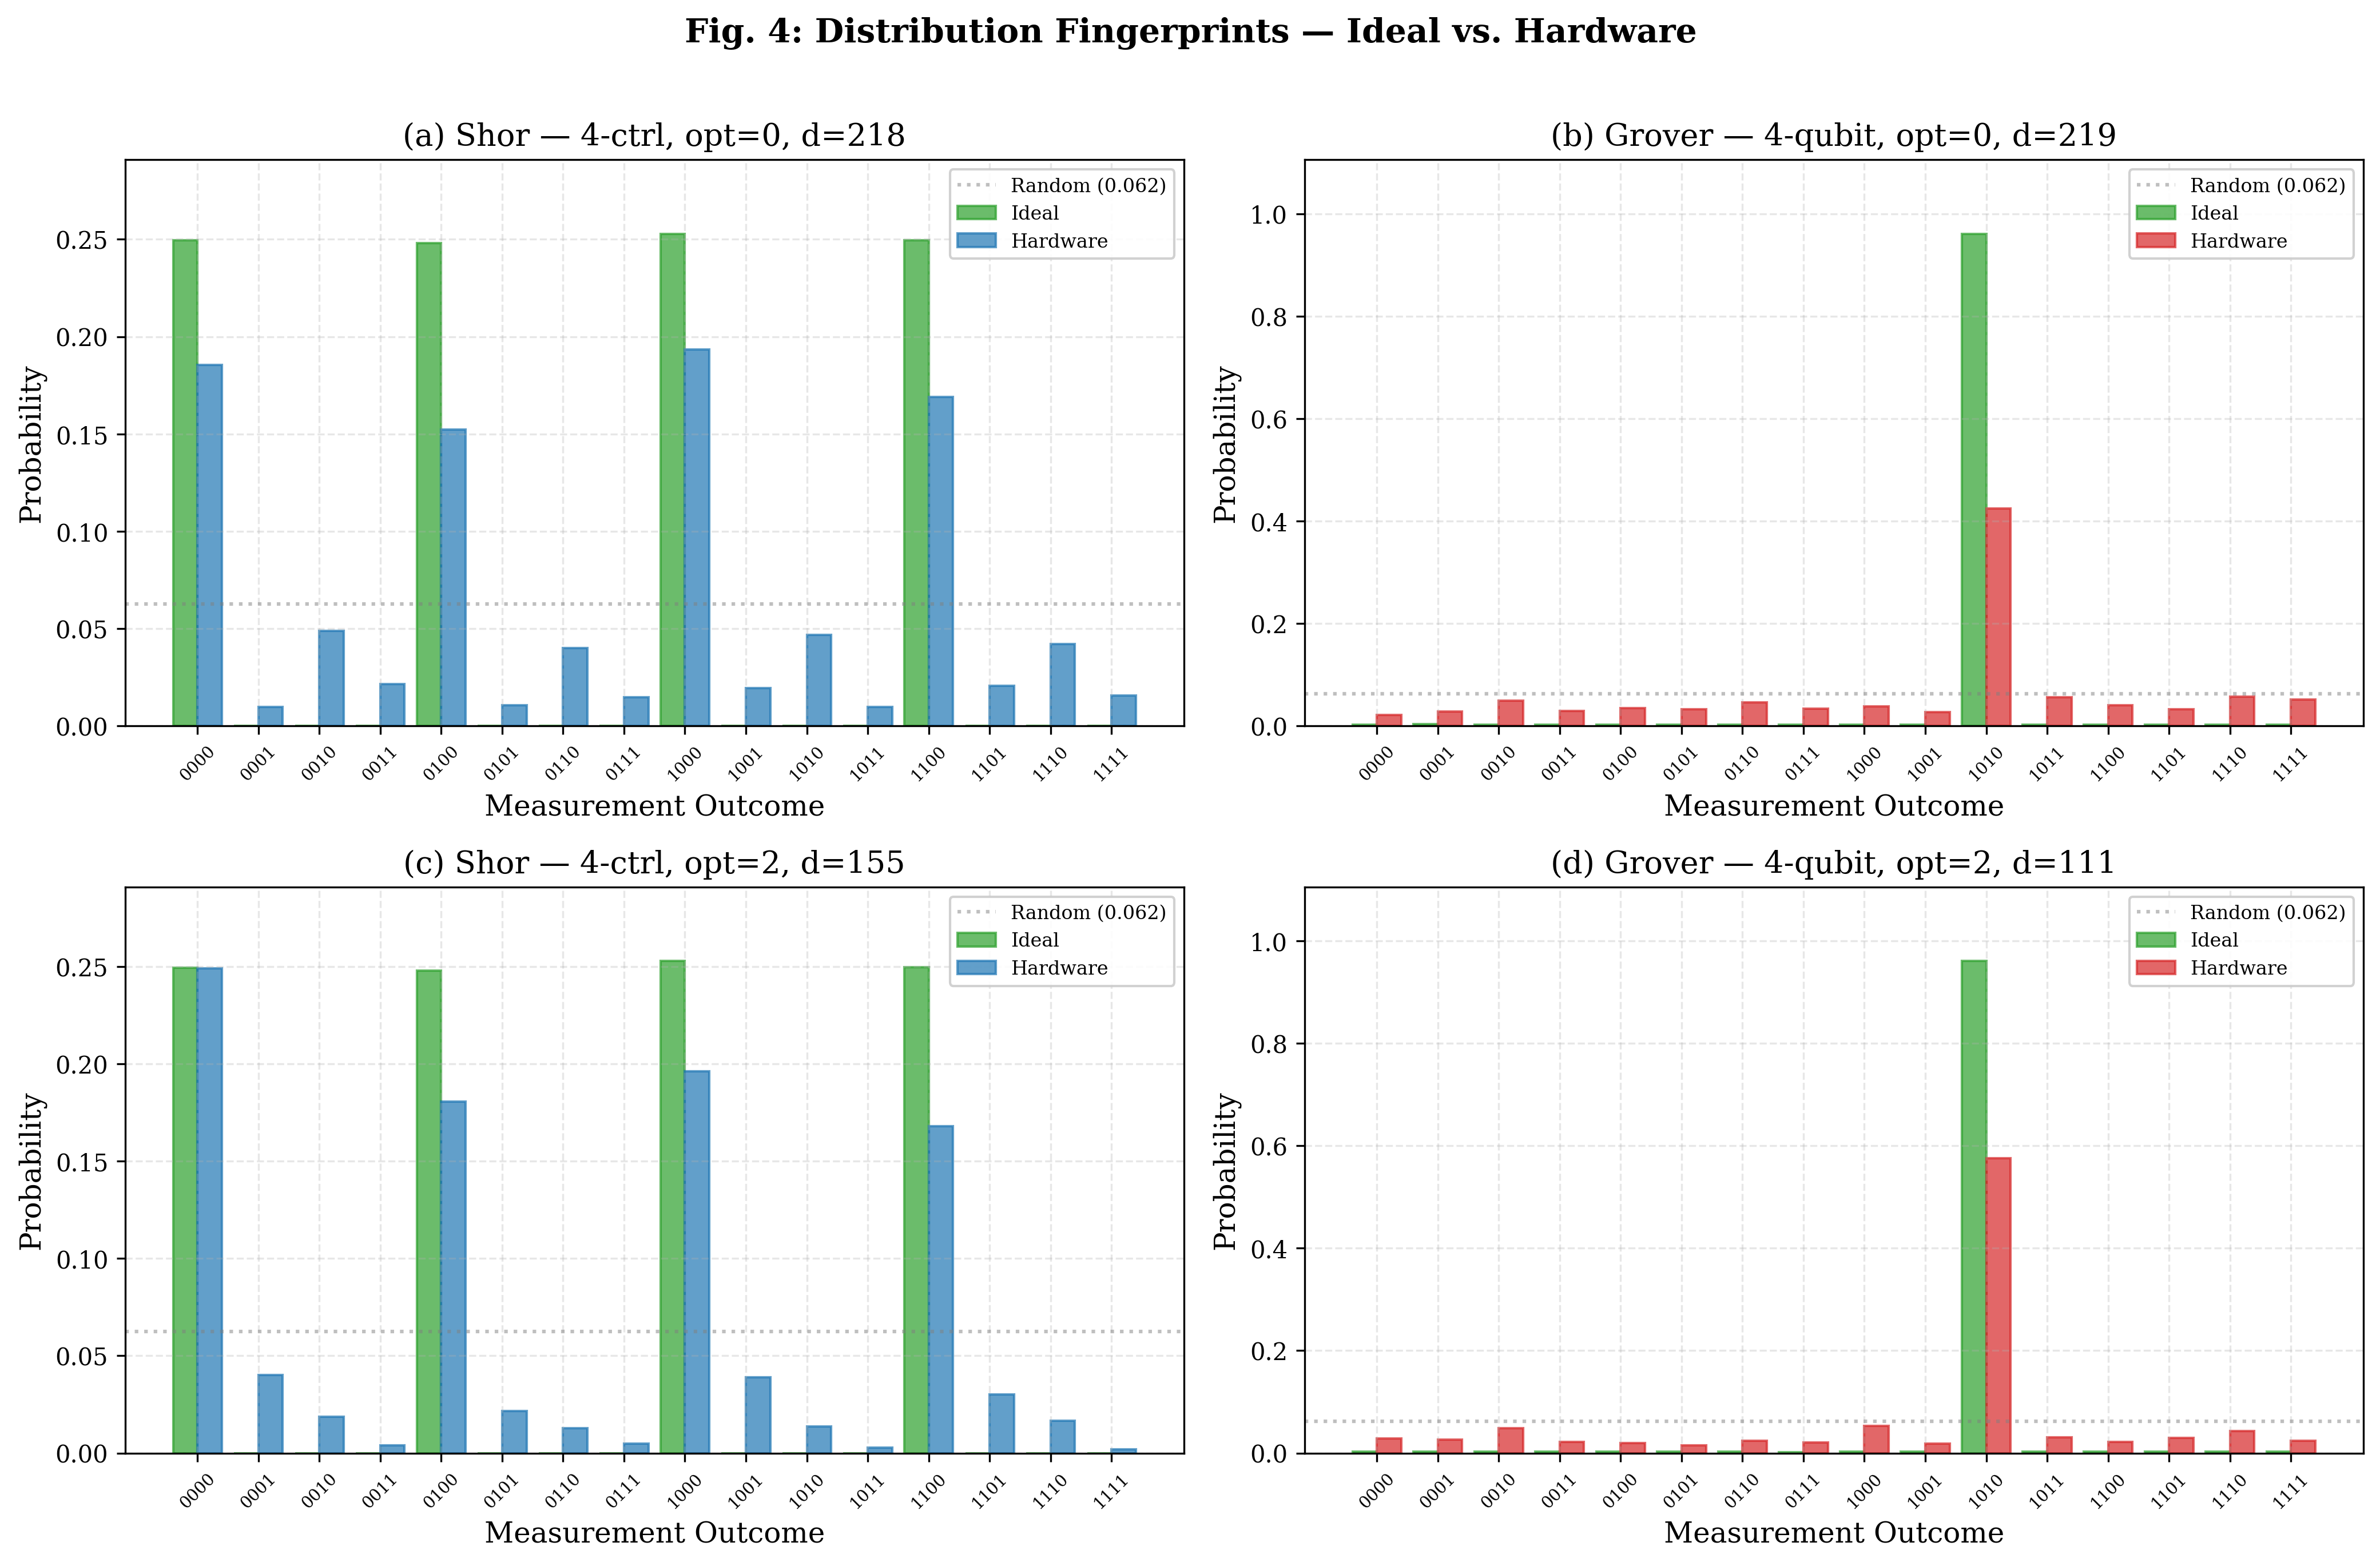
\includegraphics[width=\columnwidth]{distribution_fingerprints.png}}
\caption{Distribution fingerprints comparing ideal (green) and hardware (blue/red) probability distributions at matched circuit depths.}
\label{fig:fingerprints}
\end{figure}

\subsection{Fidelity Decay Analysis}

Fitting $p_{\text{success}} = A \cdot e^{-\lambda \cdot n_{2q}}$ to hardware success probability vs.\ two-qubit gate count yields decay constants $\lambda_S = 0.0058 \pm 0.0007$ (Shor, $R^2 = 0.79$) and $\lambda_G = 0.0048 \pm 0.0002$ (Grover, $R^2 = 0.95$). Per-gate decay rates are similar (consistent with identical hardware), but Grover starts from $A = 0.93$ (sub-unity ideal) and has zero tolerance for distributional broadening (Fig.~\ref{fig:decay}).

\begin{figure}[htbp]
\centerline{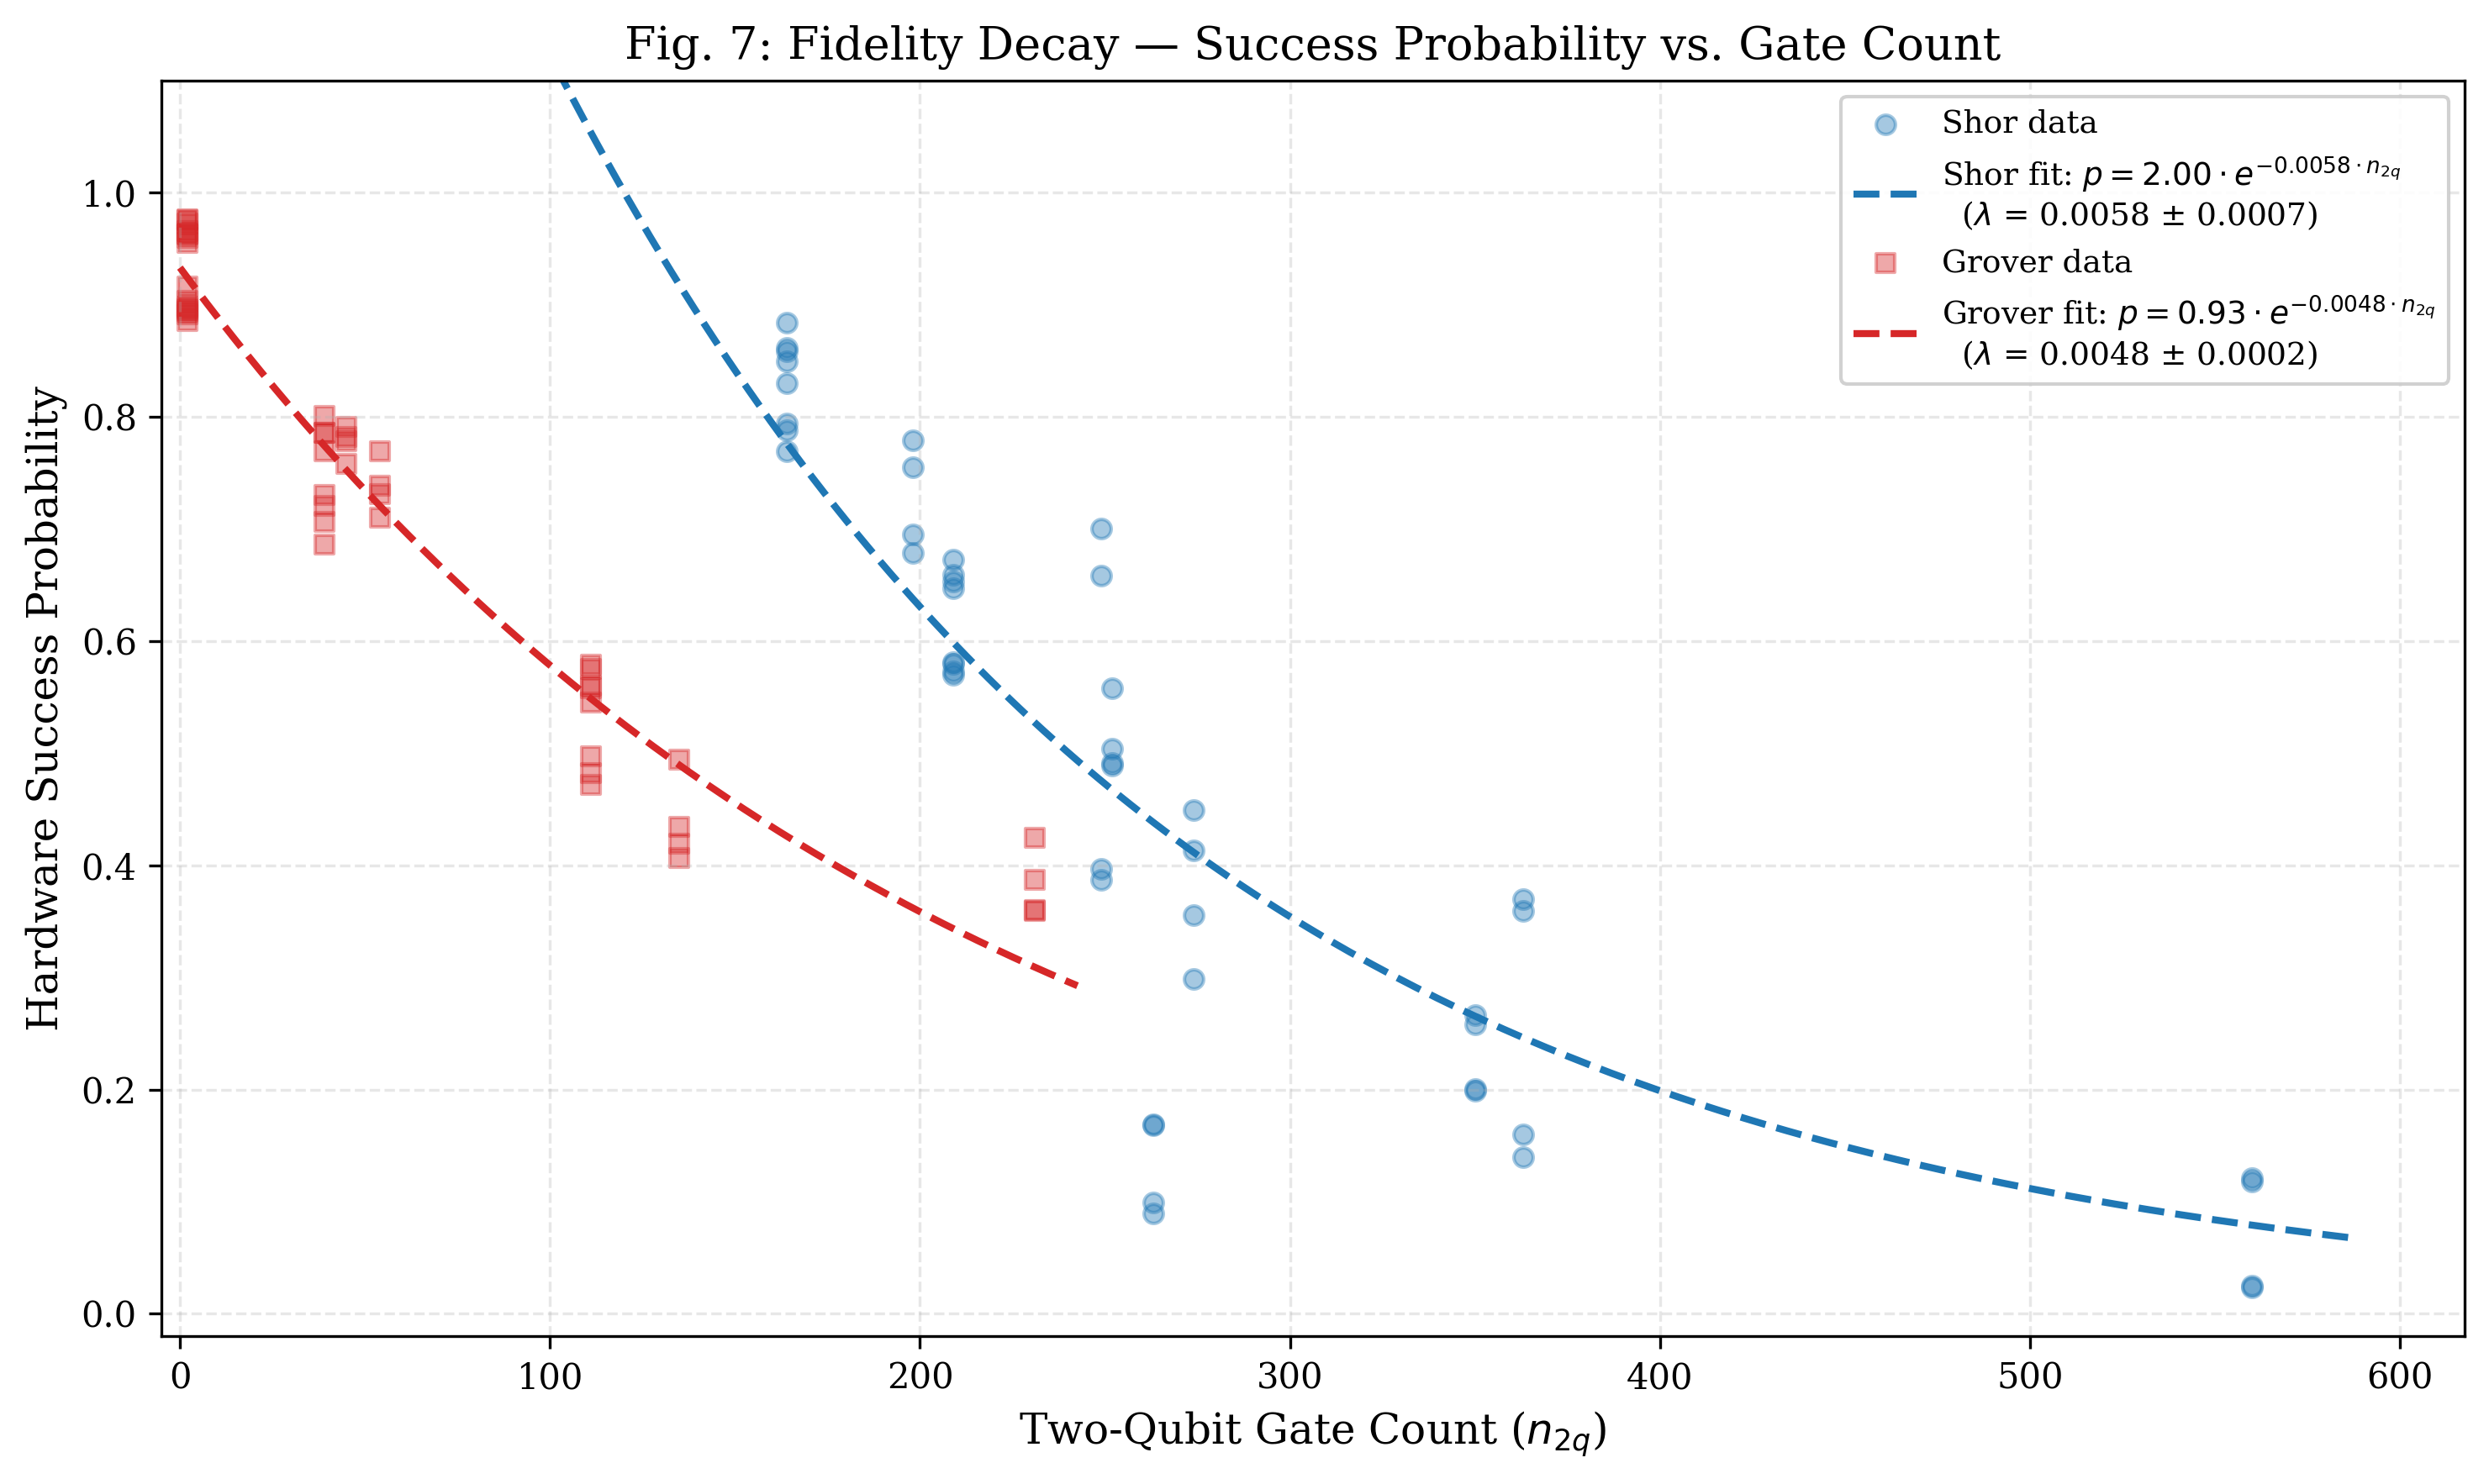
\includegraphics[width=\columnwidth]{fidelity_decay.png}}
\caption{Exponential fidelity decay: success probability vs.\ two-qubit gate count with fitted decay curves for both algorithms.}
\label{fig:decay}
\end{figure}

\subsection{Dynamical Decoupling Effectiveness}

DD provides up to +0.30 absolute improvement for deep Shor circuits at low optimization levels, where long idle periods accumulate decoherence. For Grover, DD improvements are modest ($\leq$+0.06) because the tightly-packed oracle-diffusion cycles leave fewer idle windows (Fig.~\ref{fig:dd}).

\begin{figure}[htbp]
\centerline{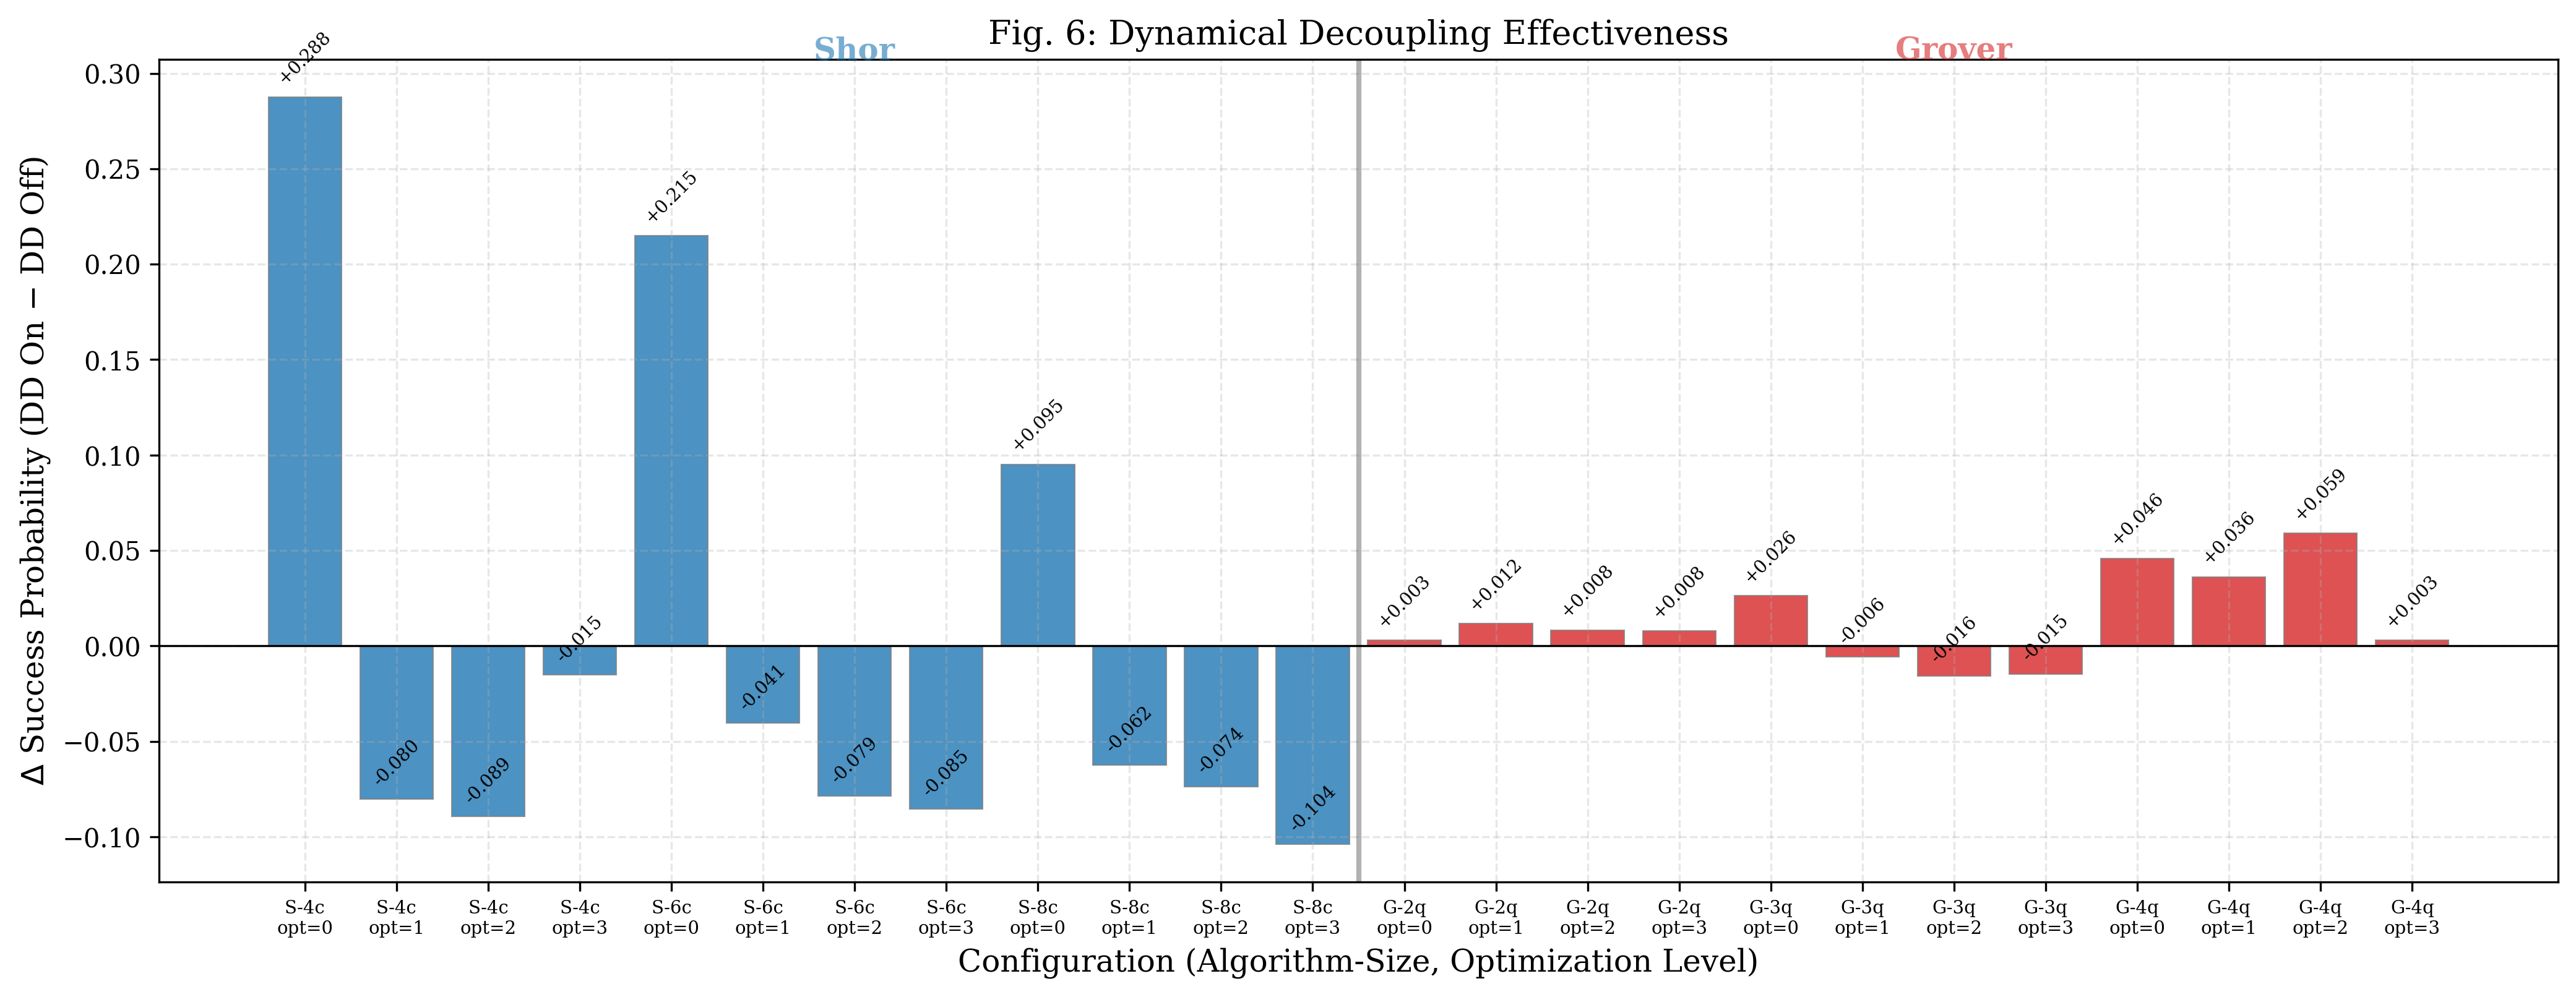
\includegraphics[width=\columnwidth]{dd_effectiveness.png}}
\caption{Dynamical decoupling effectiveness ($\Delta$ success probability) across all configurations.}
\label{fig:dd}
\end{figure}

\section{Discussion}

\subsection{Structural Origins of Differential Noise Sensitivity}

The 3.5$\times$ degradation gap is the thesis's central empirical contribution. Shor's QFT produces a \emph{multi-peaked} distribution ($r = 4$ peaks at equal probability), creating inherent redundancy: as long as peaks remain distinguishable above the noise floor, classical post-processing recovers the period. Grover's amplification concentrates probability on a \emph{single} marked state, creating a threshold degradation profile where modest noise destroys the quantum advantage entirely.

This finding is corroborated by CSU ScholarWorks (2026)~\cite{b7}, which demonstrated that applying quantum error correction (Shor's 9-qubit code) to Grover's algorithm on NISQ devices actually \emph{decreases} accuracy---the correction overhead introduces more noise than it mitigates. Our entropy efficiency data quantifies the mechanism: at $\eta_{\text{hw}} = 0.275$, Grover's 4-qubit output is already 72.5\% toward maximum entropy, leaving no headroom for correction circuits.

\subsection{Cryptographic Threat Implications}

\textbf{Public-Key Cryptography (RSA/ECC).} Shor's graceful degradation means the noise barrier is primarily a qubit-count problem. The MITRE Corporation (2025)~\cite{b8} estimated RSA-2048-breaking capability as $\sim$30 years away via Quantum Volume extrapolation. However, a March 2026 synthesis~\cite{b9} cites late-2025 algorithmic optimizations reducing the physical qubit requirement from $\sim$20M to under 1M. Our 8-control Shor data (12.1\% success at 12 qubits) provides empirical evidence for MITRE's hardware-readiness skepticism while acknowledging that algorithmic breakthroughs move the goalpost independently.

\textbf{Symmetric-Key Cryptography (AES).} Grover's 55.8\% amplification reduction at just 4 qubits compounds catastrophically at cryptographic scales. Bervice (2026)~\cite{b10} argues that Grover's speedup is practically nullified by oracle cost; our data provides the first empirical quantification of this effect. The quantum threat to AES is both a qubit-count \emph{and} a fidelity problem, pushing its timeline significantly beyond Shor's.

\subsection{Error Mitigation Landscape}

Our factorial sweep reveals transpilation optimization as the single most impactful strategy (29--49\% depth reduction, 26--35\% success improvement), followed by DD for deep circuits. SCIRP Research (2026)~\cite{b11} and Nunez et al.\ (2025)~\cite{b12} propose hybrid ZNE frameworks that extend beyond our current mitigation sweep. Our results position circuit optimization as the first line of defense before applying post-execution techniques.

A counterintuitive finding is that resilience level~1 sometimes \emph{reduces} success probability, aligning with the error correction paradox~\cite{b7}: at low $\eta_{\text{hw}}$, any correction overhead pushes the output further toward uniform noise rather than recovering the ideal signal.

\section{Challenges and Next Steps}

\textbf{Challenges.} Integrating Grover's benchmark required ensuring identical sweep dimensions and metrics conventions across both notebooks. The information-theoretic analysis required loading full probability distributions (up to 256 states per run $\times$ 3 tiers $\times$ 96 runs) rather than summary statistics, necessitating careful memory management and JSON structure design.

\textbf{Next Steps.} The remaining work comprises: (1)~completing the thesis document in Overleaf with all 7 publication-ready figures; (2)~drafting the Conclusion and Abstract chapters; (3)~supervisor review and defense preparation.

\section{Conclusion}

This report finalizes the empirical results and presents the Discussion chapter of the thesis. The cross-algorithm comparison---96 hardware runs on \texttt{ibm\_marrakesh} analyzed through both statistical and information-theoretic lenses---establishes that Grover's search algorithm is 3.5$\times$ more noise-sensitive than Shor's order-finding algorithm at comparable circuit depths. This differential, grounded in the concentrated vs.\ distributed structure of their output distributions, implies a \textbf{staggered quantum threat}: public-key cryptography (RSA/ECC) faces a nearer-term risk than symmetric-key cryptography (AES), not only because of differing qubit requirements, but because of fundamentally different noise tolerance profiles.

\begin{thebibliography}{00}
\bibitem{b1} G. Gurbanov, ``Benchmarking Shor's order-finding algorithm on IBM Quantum hardware: A three-tier comparative analysis,'' Progress Reports~1--3, Master's Thesis~II, ADA University, 2026.
\bibitem{b2} V. Bhatia and K. R. Ramkumar, ``An efficient quantum computing technique for cracking RSA using Shor's algorithm,'' in \textit{Proc. IEEE 5th Int. Conf. ICCCA}, 2020, pp. 89--94.
\bibitem{b3} P. W. Shor, ``Algorithms for quantum computation: discrete logarithms and factoring,'' in \textit{Proc. 35th Annu. Symp. Foundations of Computer Science}, 1994, pp. 124--134.
\bibitem{b4} L. K. Grover, ``A fast quantum mechanical algorithm for database search,'' in \textit{Proc. 28th Annu. ACM STOC}, 1996, pp. 212--219.
\bibitem{b5} C. Gidney and M. Eker\aa, ``How to factor 2048 bit RSA integers in 8 hours using 20 million noisy qubits,'' \textit{Quantum}, vol.~5, p.~433, 2021.
\bibitem{b6} NIST, ``Post-quantum cryptography standardization,'' FIPS 203, 204, 205, 2024.
\bibitem{b7} CSU ScholarWorks, ``Empirical evaluation of quantum error correction on Grover's algorithm in NISQ devices,'' Colorado State University, 2026.
\bibitem{b8} MITRE Corporation, ``Quantum computing threat timeline assessment via Quantum Volume extrapolation,'' Jan. 2025.
\bibitem{b9} ``Securing cryptography in the age of quantum computing and AI: threats, implementations, and strategic response,'' \textit{arXiv:2603.06969v1}, Mar. 2026.
\bibitem{b10} Bervice, ``On the practical limitations of Grover's algorithm for symmetric-key cryptanalysis,'' Feb. 2026.
\bibitem{b11} ``A novel hybrid quantum framework for assessing noise effects on performance of Shor's algorithm,'' \textit{Scientific Research Publishing}, 2026.
\bibitem{b12} D. Nunez \textit{et al.}, ``Refining noise mitigation in NISQ hardware through Qubit Error Probability,'' \textit{ResearchGate}, 2025.
\end{thebibliography}

\end{document}
